% Companion manuscript — "Digital ontogeny" (the E5+E6 arc).
% Vehicle decision 2026-07-29 (user): companion = the full E5+E6 paper;
% main_nature.tex keeps the mechanism scope + surgical deltas only.
% House rule: every number from a committed jsonl (results/e5_full/,
% results/e6_{screen,tier1,tier3,branches,microgrid,d1}/); figures from
% make_fig_ont_arc.py. Claim language per E6_SPEC locked-language +
% post-close adversarial amendments (ad17a2a, 508f502).
% Compile: latexmk -pdf companion_ontogeny
\documentclass[sn-nature]{sn-jnl}

\usepackage{graphicx}
\usepackage{booktabs}
\usepackage{amsmath,amssymb,amsfonts}
\usepackage{xcolor}
\usepackage{manyfoot}
\usepackage[font=small,labelfont=bf]{caption}
\DeclareCaptionLabelSeparator{bar}{ \textbar\ }
\captionsetup{labelsep=bar}

\begin{document}

\title[Digital ontogeny]{Digital ontogeny: a closing plasticity window in an
always-learning agent, and the one-term regularizer that abolishes it}

%\author{...}  % author block deferred to submission

\abstract{Deployed learning systems separate acting from learning; a
tropical predictive-coding substrate collapses the two into one
multiply-free pass (companion mechanism paper). Here we ask what such a
process becomes when it simply lives. Agents ran uninterrupted twelve-million-step
lives across three procedurally generated worlds --- with no replay
buffer, no rebirth, and kill-safe bit-exact resumption --- including a novel
sparse-reward world injected at seven million steps. Untreated, every mature
agent failed the novel world absolutely: zero return and zero acting entropy
across eight independent lives at two scales and two learning-rate schedules,
traced to action-readout saturation whose greedy decision core froze,
bitwise, five million steps before arrival. A pre-registered
checkpoint-branch experiment showed the one natural entropy recovery is
driven by surprise load, not semantic novelty. A single forward-KL
regularizer toward the uniform policy --- applied to the learner, not the
actor, at a calibrated dose --- abolished the age penalty: treated adults
acquired the novel world at parity with matched-treatment newborns, where
acting-time exploration noise alone recovered nothing. The cure leaves
cross-world interference untouched: serve-only re-exposure recovers none of
a displaced world model, while gradients recover it two orders of magnitude
faster than first learning. Ontogeny here delivers a durable organism whose
acquisition is age-blind; accumulation across worlds remains the measured,
mapped frontier.}

\keywords{continual learning, predictive coding, plasticity, critical
periods, reinforcement learning, neuromorphic computing}

\maketitle

\section*{Introduction}

Large language models accumulate capability by shuffling time away:
independent, identically distributed sampling lets every gradient step draw
on the whole of experience. An embodied agent is denied that trick. It meets
the world in order, once, and must remain plastic while it acts. The
companion mechanism paper establishes a substrate built for that regime ---
a tropical predictive-coding process in which serving an input and learning
from it are one multiply-free computation, exact with respect to
backpropagation, and stable over a ten-million-example text life on a single
device. This paper reports what happened when we let that process live.

We follow a single experimental object across two campaigns: a
\emph{life} --- one agent, one birth, twelve million environment steps across
alternating residencies (``eras'') in three worlds, learning on every step
from its own lived stream, with no replay buffer, no train/deploy split, and
no rebirth. The E5 campaign ran one such life and observed three phenomena
nobody designed: a fast/slow dissociation between world-model and policy
that assigns opposite plasticity roles depending only on reward signal; a
greedy decision core that froze bitwise partway through life; and a
critical-period-like failure in which the mature agent could not ignite a
policy in a novel sparse-reward world its own world model absorbed in a
single era. The E6 campaign turned those observations into a causal chain
with roughly sixty-five pre-registered lives: replicating the pathology,
isolating its mechanism and its natural counter-process by falsifier
experiments, curing it with a one-term regularizer whose dose was calibrated
by screen, and then --- via the control our own adversarial review demanded
--- correcting the cure's attribution. Every bar was frozen before launch;
every deviation is declared in the archived specification; every number in
this paper derives from committed telemetry.

\section*{Results}

\subsection*{A life, and the window that closes}

\textbf{The organism.} Lives are kill-resumable (bit-exact state capture
including environment internals and RNG streams; a deliberate kill-9 drill
is part of the operations bar), tamper-evidently ledgered, and cheap:
a full twelve-million-step, three-world life costs roughly eight dollars of
commodity CPU. Across all campaigns no life diverged, relapsed into
degenerate behaviour, or lost data; late-life capability never collapsed
under always-on plasticity. We initially reported a stronger claim --- that
capability \emph{climbs} late in life --- and retract it here: across
$n{=}3$ full baseline lives plus a fixed-learning-rate control, one life
climbed, one peaked mid-life, one was mixed. The robust lifetime claim is
\emph{maintenance without collapse}.

\textbf{The arrival pathology.} At seven million steps a fourth-world slot
opens: BabyAI-class sparse-reward gridworlds, reserved in the agent's token
vocabulary since birth but never lived. Untreated mature agents fail it
absolutely (Fig.~\ref{fig:arrival}a): return exactly zero and acting entropy
exactly zero over every lived era --- eight independent lives, two scales,
both the cycle-decayed and a fixed learning-rate schedule. A from-scratch
cohort ignites on the same world under the same recipe, so the failure is
maturity-linked, not task-impossibility. The mechanism is measured, not
inferred: the tropical action readout's top-1/top-2 logit margins grow to
19--37 nats over the first two million steps, after which the greedy action
core is \emph{bitwise frozen} --- verified by a sensitivity-audited probe
(row-permutation drives agreement to zero; the real model never moves) ---
and sampling at fixed temperature from margins that large is deterministic.
Exploration is dead on arrival, and sparse-reward learning starves without
goal contact.

\subsection*{Surprise load, not novelty, restores entropy}

E5's single life contained one natural recovery: after the novel world's
first era, the previously entropy-locked resident world regained acting
entropy and posted record returns. Two readings compete: novelty as
restorative, or mere trunk adaptation under surprising input. A
pre-registered three-arm falsifier separated them
(Fig.~\ref{fig:branch}). From one checkpoint at an entropy lock, the same
life was branched into: its natural continuation (novel world next); an
\emph{extra familiar} residency in the novelty slot; and a
\emph{scrambled} arrival --- the novel world's observation symbols permuted
so the stream is statistically surprising but semantically unlearnable (the
branch earned zero return and zero entropy in it). Result: the scrambled arm
restored downstream entropy as fully as the natural arm (0.78 vs 0.67 nats);
the familiar arm did not (0.02). Semantic, learnable novelty is unnecessary;
elapsed eras are insufficient; \emph{surprise load driving world-model
adaptation} is the operative cause. We note a residual confound this design
cannot exclude --- both restored arms were zero-reward eras while the
familiar arm retained dense reward --- and register the follow-up
(a scrambled arm with the action readout frozen) in the specification.

\subsection*{A forward-KL regularizer abolishes the age penalty}

\textbf{The cure and its control.} If saturation kills arrival learning,
desaturation should restore it --- but where must it act? An eight-arm
pre-registered screen (five seeds per arm, compressed lives) tested three
intervention families. The decisive contrast: an acting-time exploration
floor ($\varepsilon$-mixed sampling) explores but never ignites (0/5 seeds),
while a \emph{training-time} pull of the action readout toward the uniform
policy ignites in every seed. The pull is the gradient of
$\lambda\,\mathrm{CE}(U,\pi)$ --- the \emph{forward}
Kullback--Leibler direction $D_{\mathrm{KL}}(U\Vert\pi)$, which diverges as
any action's probability approaches zero and therefore concentrates its
restoring force exactly on saturation. The term itself is inherited, not
new: it is label smoothing's gradient\cite{szegedy2016}, the KL form of
DreamerV3's `unimix'\cite{hafner2023dreamer}, and the log-barrier
regularizer of ref.~\citenum{agarwal2021pg}; the maximum-entropy
tradition\cite{ziebart2008,haarnoja2018sac} and the confidence
penalty\cite{pereyra2017} use the \emph{reverse} direction, whose
restoring force does not concentrate on dying
actions\cite{meister2020}. What is new here is the isolation of the
direction as the operative ingredient of a plasticity rescue, and the
locus: it is one shift-class term in the existing learning pass, costing
no additional forward computation. Dose
matters monotonically: at $\lambda=2^{-3}$ ignition costs resident-world
performance; at $2^{-4}$ the screen's no-tax bar is met in both resident
worlds (Fig.~\ref{fig:dose}).

\textbf{Full scale, and the corrected attribution.} At full scale ---
twelve-million-step lives, arrival at seven million with twice the screen's
saturation history --- treated adults ignited in six of six lives across
both doses; at the calibrated dose their arrival returns (3.12/3.37/3.02
per thousand steps) initially read \emph{above} the historical newborn
cohort. Our adversarial review demanded the obvious control, and it ruled
against the romantic reading: a twenty-life newborn grid showed the pull
helps newborns too (untreated 2.08, treated 3.35 on matched fresh worlds),
and gentler learning rates alone also help. Under matched treatment,
maturity is \emph{neutral}: treated adults perform at parity with treated
newborns (Fig.~\ref{fig:arrival}b). The correct statement --- and, against
an absolute zero baseline in eight untreated lives, we believe the important
one --- is that the regularizer \emph{abolishes the age penalty}: acquisition
becomes age-blind. Treated adults also retain the novel-world skill across
all subsequent revisits (nine of nine revisit eras at or above their arrival
level), with acting entropy alive throughout.

\subsection*{What the cure does not buy: the accumulation frontier}

The cure leaves cross-world interference untouched (non-resident world-model
probe error changes by $-0.2\%$; Fig.~\ref{fig:seesaw}): acquisition and
accumulation are mechanistically orthogonal. Two further pre-registered
results locate the remaining frontier precisely. First, protection-type
consolidation fails its bars: an elastic-weight anchor\cite{kirkpatrick2017} reduces non-resident
error by only 10\% against a 30\% bar while taxing novel-world plasticity,
and per-weight meta-learned step sizes (three IDBD\cite{sutton1992} variants at
$\theta{=}0.01$) worsen both sides --- a scoped negative with a registered
retry map, since our own review diagnosed the tested meta-rate as
pathologically fast. Second, a branch-freeze discriminator classified the
interference itself (Fig.~\ref{fig:freeze}): fifty thousand serve-only steps
back in a familiar world recover \emph{nothing} (instantaneous prediction
error flat at 19--22 nats), while restored gradients recover twenty nats in
one to three thousand steps --- roughly a hundredfold faster than first
acquisition. Features are preserved; the output mapping is displaced;
remapping requires updates. This kills calibration-style remedies and
selects the structural class --- slow-trunk/fast-adapter separations, sparse
modular routes, or low-rank subspace protection --- as the accumulation
arc's search space.

\section*{Discussion}

Three claims survive this arc's own hostile review cleanly. A
\emph{systems existence proof}: an always-learning, replay-free,
single-process organism lives multi-world lives at fleet scale with
auditable operations and no stability failures. A \emph{developmental
dissociation}: within one substrate, world-model and policy take opposite
plasticity roles set by reward signal --- the world model acquires a novel
world in one era at decayed learning rates while the policy is frozen; the
policy retains mastered skills open-loop while the world model's storage is
displaced beneath it. And a \emph{causal account of the closing window}:
saturation-driven, surprise-restorable, and abolishable by one forward-KL
term at the learner --- with the honest boundary that this solves
acquisition, not accumulation. We position these claims carefully against
their neighbours. Loss of plasticity and its remedies are established
\cite{dohare2024,sokar2023,nikishin2023,juliani2024}; to our knowledge no
reported cure reaches \emph{parity with a fresh network} on new-task
acquisition under matched treatment, as here. Critical-period analyses in
artificial networks treat closure as effectively
irreversible\cite{achille2019}; we reopen a closed window with a loss
term rather than surgery or resets --- an analogy, not a mechanism claim,
to biological reopening\cite{pizzorusso2002}. Suppression-versus-erasure
and savings phenomena are known\cite{davari2022,hetherington1989}; our
contribution is the zero-gradient discriminator that separates them in a
live organism and the quantified $\sim$100$\times$ savings. And
surprise-driven exploration is the premise of intrinsic
motivation\cite{burda2019}; the scrambled$\approx$natural cross-task
restoration dissociation has, to our knowledge, no located precedent.

We are explicit about scope. The worlds are small and the skills mostly
disjoint; per-skill competence is the right unit, and ``acquires the world''
means its dominant levels. The lifetime-gain property that would make such
an organism economically interesting --- compounding, LLM-like accumulation
over ordered experience --- is measured here only as its precondition
(maintenance) and its obstacle (displacement-type interference), with the
remedy class selected but unbuilt. The substrate's silicon claims live in
the companion paper; nothing in this arc required them, and the cure's
shift-class arithmetic ports to that hardware unchanged.

What ontogeny has delivered, in the end, is a subject: an organism durable
enough to experiment on, instrumented enough to be honest about, and now
old enough to learn like the young. Whether it can be made to \emph{grow}
--- to leave each world richer for the next --- is the single question the
next arc exists to answer.

\section*{Methods summary}

Agents are 77k-parameter, four-layer tropical state-space models with a
separate top-$k$ action readout, trained by cascade predictive-coding credit
assignment (bitwise-equivalent to backpropagation; companion paper) on
policy-as-token-prediction with windowed REINFORCE credit, intrinsic
surprise shaping and advantage normalization, updating on every step.
Worlds: a procedural foraging gridworld, MinAtar, and BabyAI-class
fixed-mission levels, alternating in 250k--500k-step eras with intra-era
biome rotation; environments never reset across a life. Probes are
clone-isolated (state-hash-audited) suites over frozen windows and
fixed-seed clone episodes. All experiment bars were pre-registered and
frozen before launch (archived specification with in-line amendments);
lives are bit-exact resumable, and a flags-off code path is verified
bitwise-identical against the pre-campaign commit. Data: every figure
derives from committed telemetry in the public archive
(\texttt{results/e5\_full}, \texttt{results/e6\_*}); the analysis and
figure code, the full specification with its adversarial-review amendments,
and per-life ledgers are versioned alongside. External adversarial review
(an independent frontier model consulted by the authors) shaped the
KL-direction framing, the dose design, the freeze discriminator, and two
attribution corrections; all four contributions are logged in the archive.

\begin{figure}
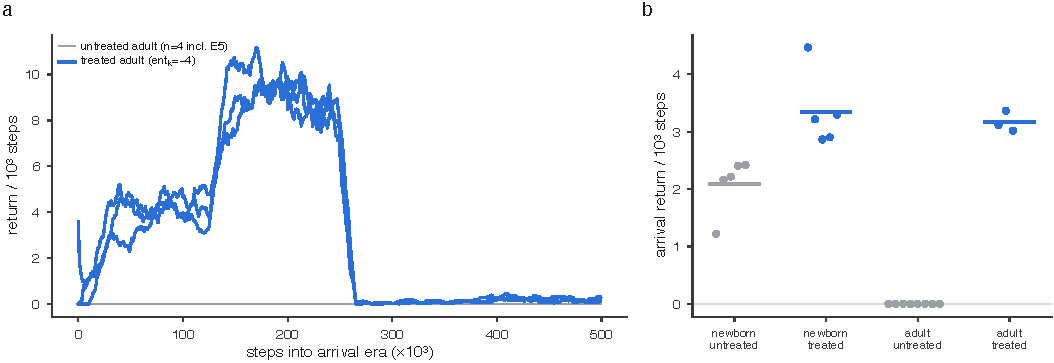
\includegraphics[width=\textwidth]{figs/fig_ont_arrival.pdf}
\caption{\textbf{The arrival pathology and the abolished age penalty.}
\textbf{a}, Return trajectories through the novel world's first era
(smoothed, per-thousand-step returns) for untreated full-scale adults
(grey; $n{=}4$ lives shown, all identically zero) and adults treated with
the calibrated forward-KL pull (blue; $n{=}3$).
\textbf{b}, Matched-treatment comparison: whole-run returns for untreated
and treated newborns (five fresh-world seeds each; horizontal bars, means)
against untreated adults (eight lives, all zero) and treated adults
($n{=}3$). Treatment, not maturity, separates the groups: the pull helps
newborns too, and under matched treatment maturity is neutral.}
\label{fig:arrival}
\end{figure}

\begin{figure}
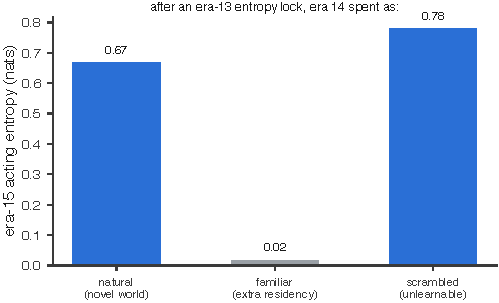
\includegraphics[width=0.6\textwidth]{figs/fig_ont_branch.pdf}
\caption{\textbf{Surprise load, not novelty, restores entropy.} From one
checkpoint at an entropy lock, three branched continuations of the same
life: the natural novel-world era, an extra familiar residency, and a
scrambled (statistically novel, unlearnable) era. Downstream resident-world
acting entropy recovers only where surprise load was high --- including the
arm in which nothing could be learned.}
\label{fig:branch}
\end{figure}

\begin{figure}
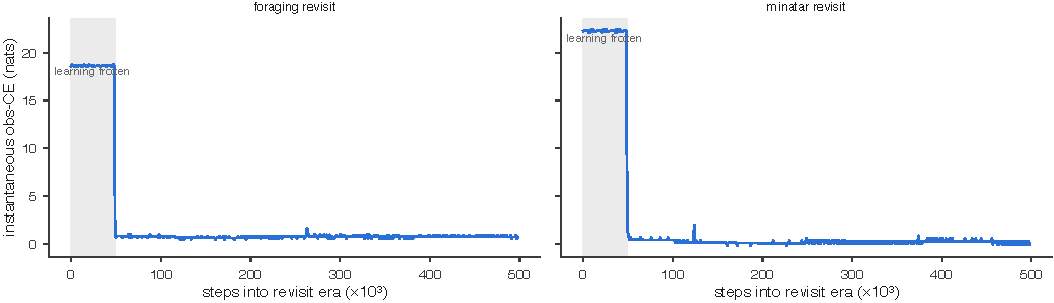
\includegraphics[width=\textwidth]{figs/fig_ont_freeze.pdf}
\caption{\textbf{Displacement, not shadowing.} Instantaneous world-model
prediction error through revisit eras whose first fifty thousand steps ran
serve-only (shaded): re-exposure without updates recovers nothing in either
world; restored gradients recover $\sim$20 nats within one to three
thousand steps.}
\label{fig:freeze}
\end{figure}

\begin{figure}
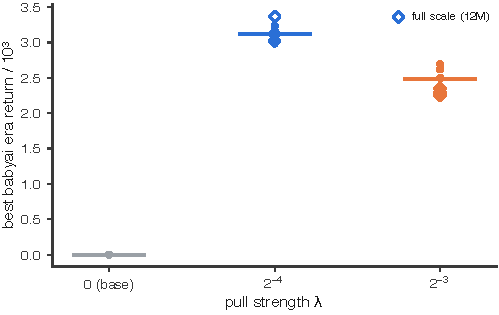
\includegraphics[width=0.55\textwidth]{figs/fig_ont_dose.pdf}
\caption{\textbf{Dose--response of the forward-KL pull.} Best novel-world
era return per life versus pull strength, at screen scale (dots) and full
scale (diamonds). Ignition is robust at both non-zero doses; resident-world
taxes (main text) select $\lambda{=}2^{-4}$.}
\label{fig:dose}
\end{figure}

\begin{figure}
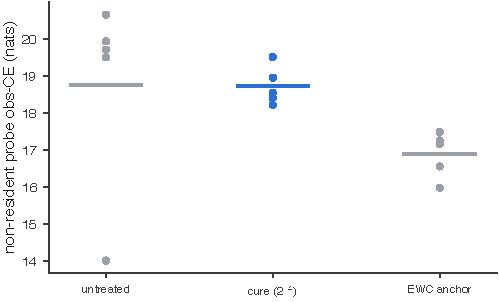
\includegraphics[width=0.55\textwidth]{figs/fig_ont_seesaw.pdf}
\caption{\textbf{The cure does not touch interference.} Mean non-resident
world-model probe error per life, by arm: the calibrated cure is
indistinguishable from baseline (the acquisition and accumulation problems
are orthogonal); the elastic-weight anchor's modest reduction fails its
pre-registered bar.}
\label{fig:seesaw}
\end{figure}

\begin{thebibliography}{99}
\bibitem{szegedy2016} Szegedy, C. et al. Rethinking the Inception
architecture for computer vision. \emph{CVPR} (2016).
\bibitem{hafner2023dreamer} Hafner, D. et al. Mastering diverse domains
through world models. \emph{arXiv:2301.04104} (2023).
\bibitem{agarwal2021pg} Agarwal, A., Kakade, S., Lee, J. \& Mahajan, G.
On the theory of policy gradient methods. \emph{JMLR} \textbf{22} (2021).
\bibitem{ziebart2008} Ziebart, B. et al. Maximum entropy inverse
reinforcement learning. \emph{AAAI} (2008).
\bibitem{haarnoja2018sac} Haarnoja, T. et al. Soft actor--critic.
\emph{ICML} (2018).
\bibitem{pereyra2017} Pereyra, G. et al. Regularizing neural networks by
penalizing confident output distributions. \emph{ICLR workshop} (2017).
\bibitem{meister2020} Meister, C., Salesky, E. \& Cotterell, R.
Generalized entropy regularization. \emph{ACL} (2020).
\bibitem{dohare2024} Dohare, S. et al. Loss of plasticity in deep
continual learning. \emph{Nature} \textbf{632} (2024).
\bibitem{sokar2023} Sokar, G. et al. The dormant neuron phenomenon in
deep reinforcement learning. \emph{ICML} (2023).
\bibitem{nikishin2023} Nikishin, E. et al. Deep reinforcement learning
with plasticity injection. \emph{NeurIPS} (2023).
\bibitem{juliani2024} Juliani, A. \& Ash, J. A study of plasticity loss
in on-policy deep reinforcement learning. \emph{NeurIPS} (2024).
\bibitem{achille2019} Achille, A., Rovere, M. \& Soatto, S. Critical
learning periods in deep networks. \emph{ICLR} (2019).
\bibitem{pizzorusso2002} Pizzorusso, T. et al. Reactivation of ocular
dominance plasticity in the adult visual cortex. \emph{Science}
\textbf{298} (2002).
\bibitem{davari2022} Davari, M. et al. Probing representation forgetting
in supervised and unsupervised continual learning. \emph{CVPR} (2022).
\bibitem{hetherington1989} Hetherington, P. \& Seidenberg, M. Is there
`catastrophic interference' in connectionist networks? \emph{CogSci}
(1989).
\bibitem{burda2019} Burda, Y. et al. Exploration by random network
distillation. \emph{ICLR} (2019).
\bibitem{kirkpatrick2017} Kirkpatrick, J. et al. Overcoming catastrophic
forgetting in neural networks. \emph{PNAS} \textbf{114} (2017).
\bibitem{sutton1992} Sutton, R. S. Adapting bias by gradient descent: an
incremental version of delta-bar-delta. \emph{AAAI} (1992).
\end{thebibliography}

\end{document}
